\documentclass{beamer}

\mode<presentation>
{
  \usetheme{Antibes}
  \setbeamercovered{transparent}
  \setbeamertemplate{navigation symbols}
}

\usepackage[english]{babel}
\usepackage[latin1]{inputenc}
\usepackage{times}
\usepackage[T1]{fontenc} 
% Or whatever. Note that the encoding and the font should match. If T1
% does not look nice, try deleting the line with the fontenc.
\usepackage{amsmath}

\newcommand{\linespace}{\vskip 0.25cm}

\definecolor{MyForestGreen}{rgb}{0,0.7,0} 
\newcommand{\mynotes}[1]{}

% The text in square brackets is the short version of your title and will be used in the
% header/footer depending on your theme.
\title[Interoperability]{Interoperability in Programming Languages}

% Sub-titles are optional - uncomment and edit the next line if you want one.
% \subtitle{Why does sub-tree crossover work?} 

% The text in square brackets is the short version of your name(s) and will be used in the
% header/footer depending on your theme.
\author[Malone]{Todd Malone}

% The text in square brackets is the short version of your institution and will be used in the
% header/footer depending on your theme.
\institute[U of Minn, Morris]
{
  Division of Science and Mathematics \\
  University of Minnesota, Morris \\
  Morris, Minnesota, USA
}

% The text in square brackets is the short version of the date if you need that.
\date[April '14, Senior Sem] % (optional)
{28 April 2014 \\ Senior Seminar}

% Delete this, if you do not want the table of contents to pop up at
% the beginning of each subsection:
\AtBeginSection[]
{
  \begin{frame}<beamer>
    \frametitle{Outline}
    \tableofcontents[currentsection, hideothersubsections]
  \end{frame}
}

\begin{document}

\begin{frame}
  \titlepage
\end{frame}

% For a 20-25 minute senior seminar talk you probably want something like:
% - Two or three major sections (other than the summary).
% - At *most* three subsections per section.
% - Talk about 30s to 2min per frame. So there should probably be between
%   15 and 30 frames, all told.
% Slide notes will be comment under each frame end, or under each column where appropriate.

\section*{Introduction}

\subsection*{Defining Interoperability}

\begin{frame}
  \frametitle{What is interop?}
  
  %\begin{columns}
  %\begin{column}{0.6\textwidth}
  \begin{itemize}
  	\item Interoperability: The ability for two systems to interact.
  	\item Often shortened to interop.
	\item In programming languages: The ability of a language to call on code from another language.
  \end{itemize}
  %\end{column}
%mainly, a program running in one language has the ability to call on aspects of another program, written in a different language  
%the ability for a program written in one language to call on a program written in another lanugage.
 
  %\end{columns}
\end{frame}

\subsection*{The Importance of Interop}

\begin{frame}
  \frametitle{Why is interop important?}
%These generally fall under to main categories: Dev time, or effort; and the purpose of different languages.
  
  \begin{columns}[t]
  \begin{column}{0.5\textwidth}
  Developer time and effort:
  \begin{itemize}
	\item Existing and working code is easier to use as-is.
	\item Legacy systems: extensive or little-understood code base.
  	\item Third-party systems: source code is unavailable

  \end{itemize}
  \end{column}
  %existing (and working) code that does the thing you need it to do, it's easier to use as it is than it is to rewrite it.
  %sometimes, rewriting is an option, but there's just too much code and domain knowledge involved. (example: that a polygon doesn't cross itself) (if there's a lot, it would take a long time, too)
  %other time, you 

  \begin{column}{0.6\textwidth}
  Language Strength:
  \begin{itemize}
  	\item Explicit memory access (C)
  	\item Parallel or distributed systems (Clojure, Erlang)
  	\item Statistics (R)
  \end{itemize}
  \end{column}
  \end{columns}
%
%each of these languages has some drawbacks, which not hugely importnant
%however, if the programmer isn't comfortable enough with the language to deal with its escentricities,
%then they'd be better served by utilizing it for the specific thing they need from it, in as small a chunk as they can get.

  
\end{frame}

\subsection*{Outline}

\begin{frame}
  \frametitle{Outline}
  \tableofcontents[hideallsubsections]
\end{frame}
%I'll be talking about two particular tools used for enabling interoperability,
%as well as two particular concepts central to interop in programming languages




\section[Difficulties]{Common difficulties in interop}
%Everything in this section is closely related: it's all about the data. And differences between languages
%The three main problems encountered in 


\subsection{Type systems}
  %Primarially what languages *call* different kinds of data,
  %but also how they distinguish between similar kinds of data (such as different kinds of numbers)
\begin{frame}
  \frametitle{Differences in type systems}
  
  \begin{columns}
  \begin{column}{0.6\textwidth}
  \begin{itemize}
  	\item Languages represent data in different ways %numbers: Java says "int!", JavaScript says "Number!". Ruby says "Whatever! I'll figure it out."
	\item Statically-typed languages assign types as soon as data is collected.
	\item Dynamically-typed languages only deal with types when evaluating data.
  \end{itemize}
  \end{column}
  %One major source of difference, in all of these sections, is going to be numbers. Numbers get represented in a lot of ways, even within a single language.
  %Java, for instance, has at least four(?) ways of representing number: Integers, Doubles, Floats (similar to doubles), and BigIntegers
  %Javascript and Ruby will figure out what you mean later.
  %How do we go from "X is a thing we'll deal with when we have to" to "X is an integer, and we know what we can do with it now"?

  \begin{column}{0.5\textwidth}
  
\includegraphics[scale=1]{graphics/StrongTypeCliff.pdf}
  
  \tiny{statically-typed person}
  \linespace
  \linespace
  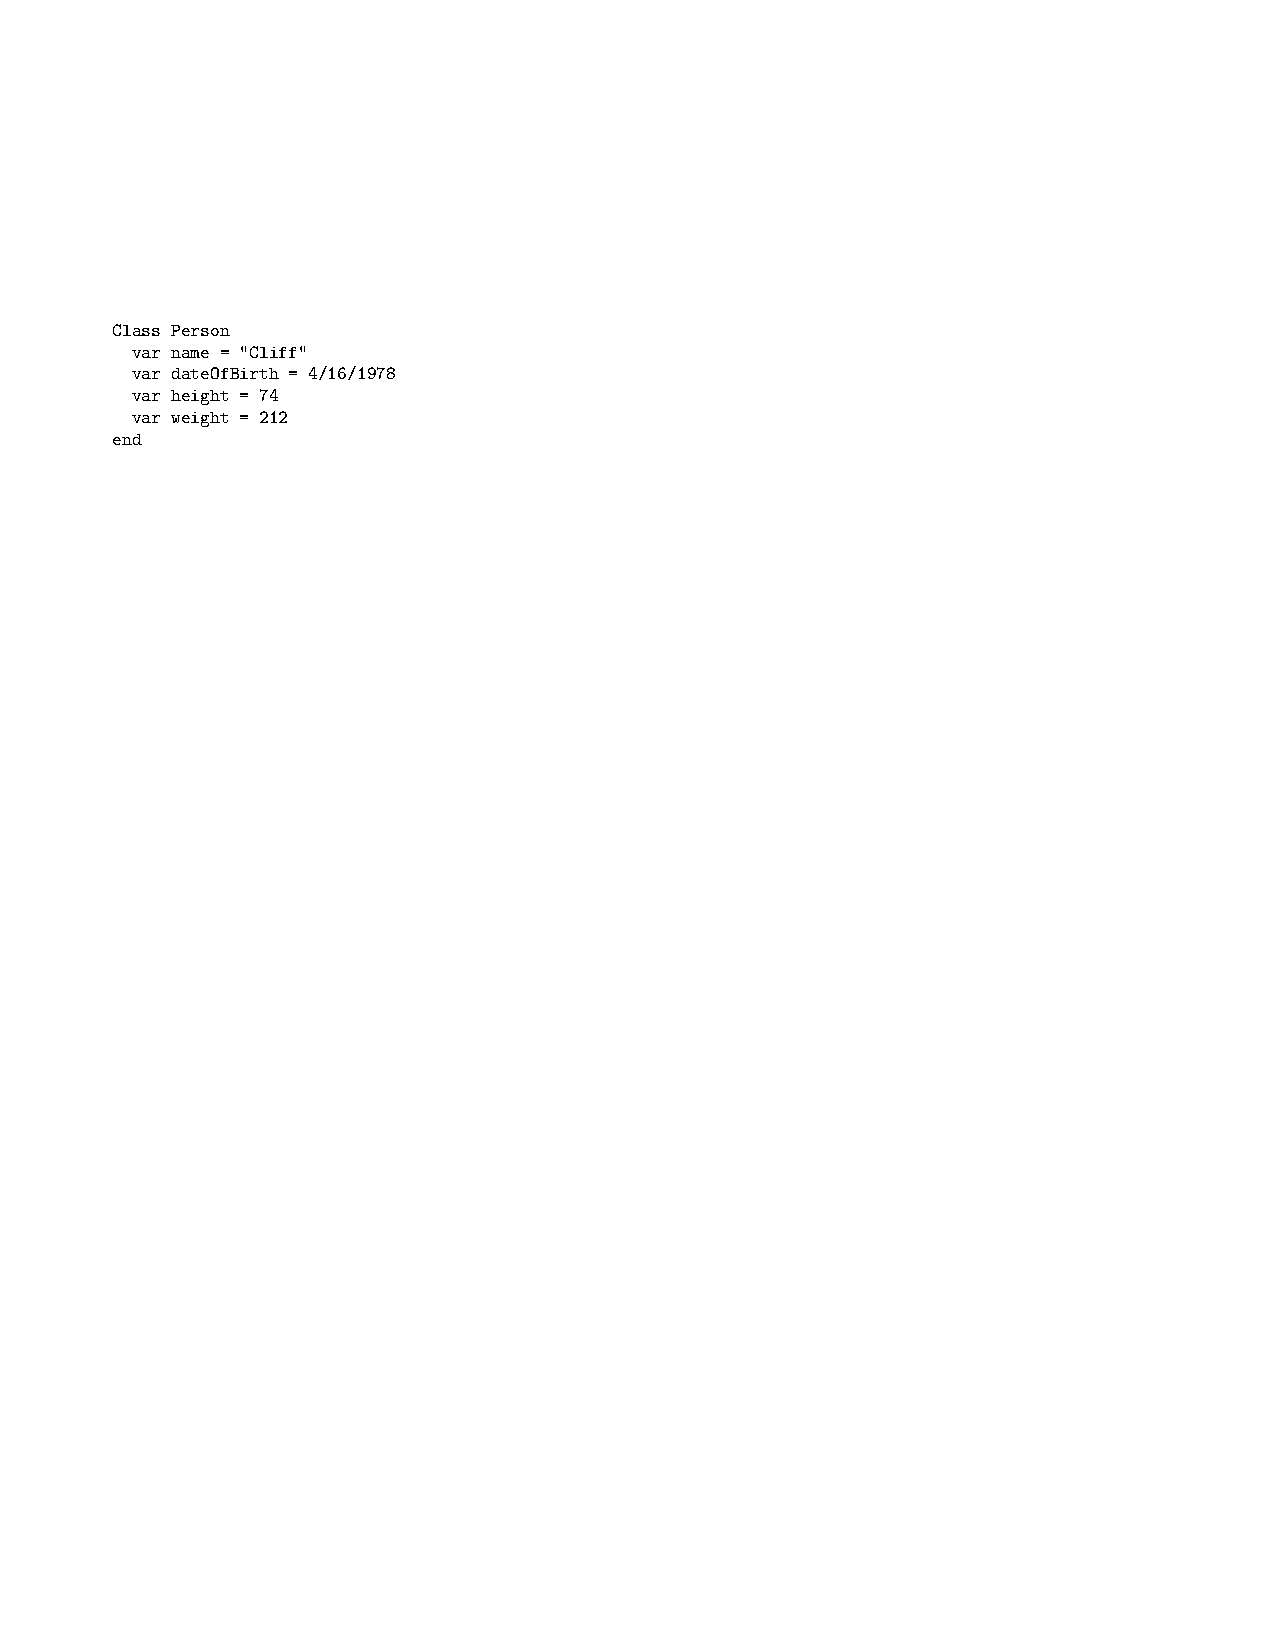
\includegraphics[scale=1]{graphics/UnTypeCliff.pdf}
  
  \tiny{dynamically-typed person}
  \end{column}
  \end{columns}
\end{frame}
%Numbers are really the easiest example, because there are so many ways of representing them. 

\subsection{Data structures}
\begin{frame}
  \frametitle{Types in data structures}
  
  \begin{columns}
  \begin{column}{0.5\textwidth}
  \begin{itemize}
  	\item Untyped lists can contain different types,
  	\item Strongly typed lists can only contain the type given by the list.
  \end{itemize}
  \end{column}
  
  \begin{column}{0.5\textwidth}
  {\tt [23, v, "hello", True]}
  
   An untyped list
\linespace   
  {\tt [1, 53, 13, 100]}
  
  a typed list 
\linespace	
  {\tt Object[] = [?, ?, ?, ?]}
  
  A Java list of Objects
  \end{column}
  \end{columns}
\end{frame}
  %A list containing strings and integers is going to be hard to map to a strongly-typed list.
  %
  %A partial example here is C, which doesn't have a notion of Key/Value maps.
  %It does have the building blocks for creating maps, and this will usually be the case. But Time and Effort!
\begin{frame}
  \frametitle{Missing data structures}
  \begin{columns}
  \begin{column}{0.5\textwidth}
  \begin{itemize}
  \item A data structure in one language may be absent in another.
  \item Any language can build any data structure, but it may be more difficult in certain languages.
  \item Building a non-native data structure takes time and effort.
  \end{itemize}
  
  \end{column}
  \begin{column}{0.6\textwidth}
  {\tt \{:name "Cliff", :age 32}\}
  
  Maps are common data structures, but absent in C.
  \end{column}
  \end{columns}
\end{frame}

\subsection{Data processing}
%In some cases, languages act differently when performing the same operations on the same data
\begin{frame}
  \frametitle{Handling data}
  
  \begin{columns}
  \begin{column}{0.5\textwidth}
  \begin{itemize}
  \item Languages act on data in different ways. %This is most obvious in numbers, but Java and C# handle printing of NULL objects very differently
  \item Handling NULL or NIL objects.
  \end{itemize}
  \end{column}
  
  \begin{column}{0.5\textwidth}
  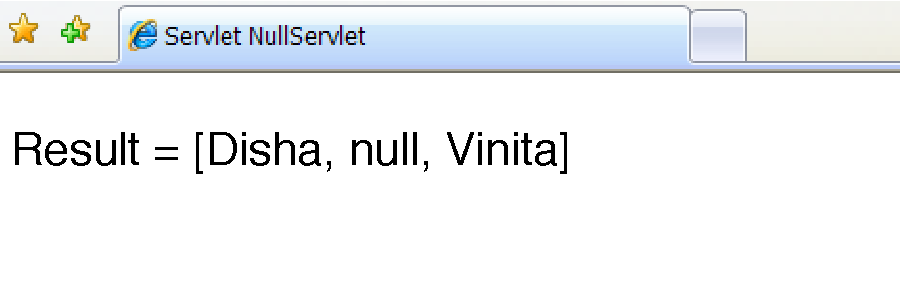
\includegraphics[scale=0.35]{graphics/modifiedJavaNull.pdf}
  \linespace
  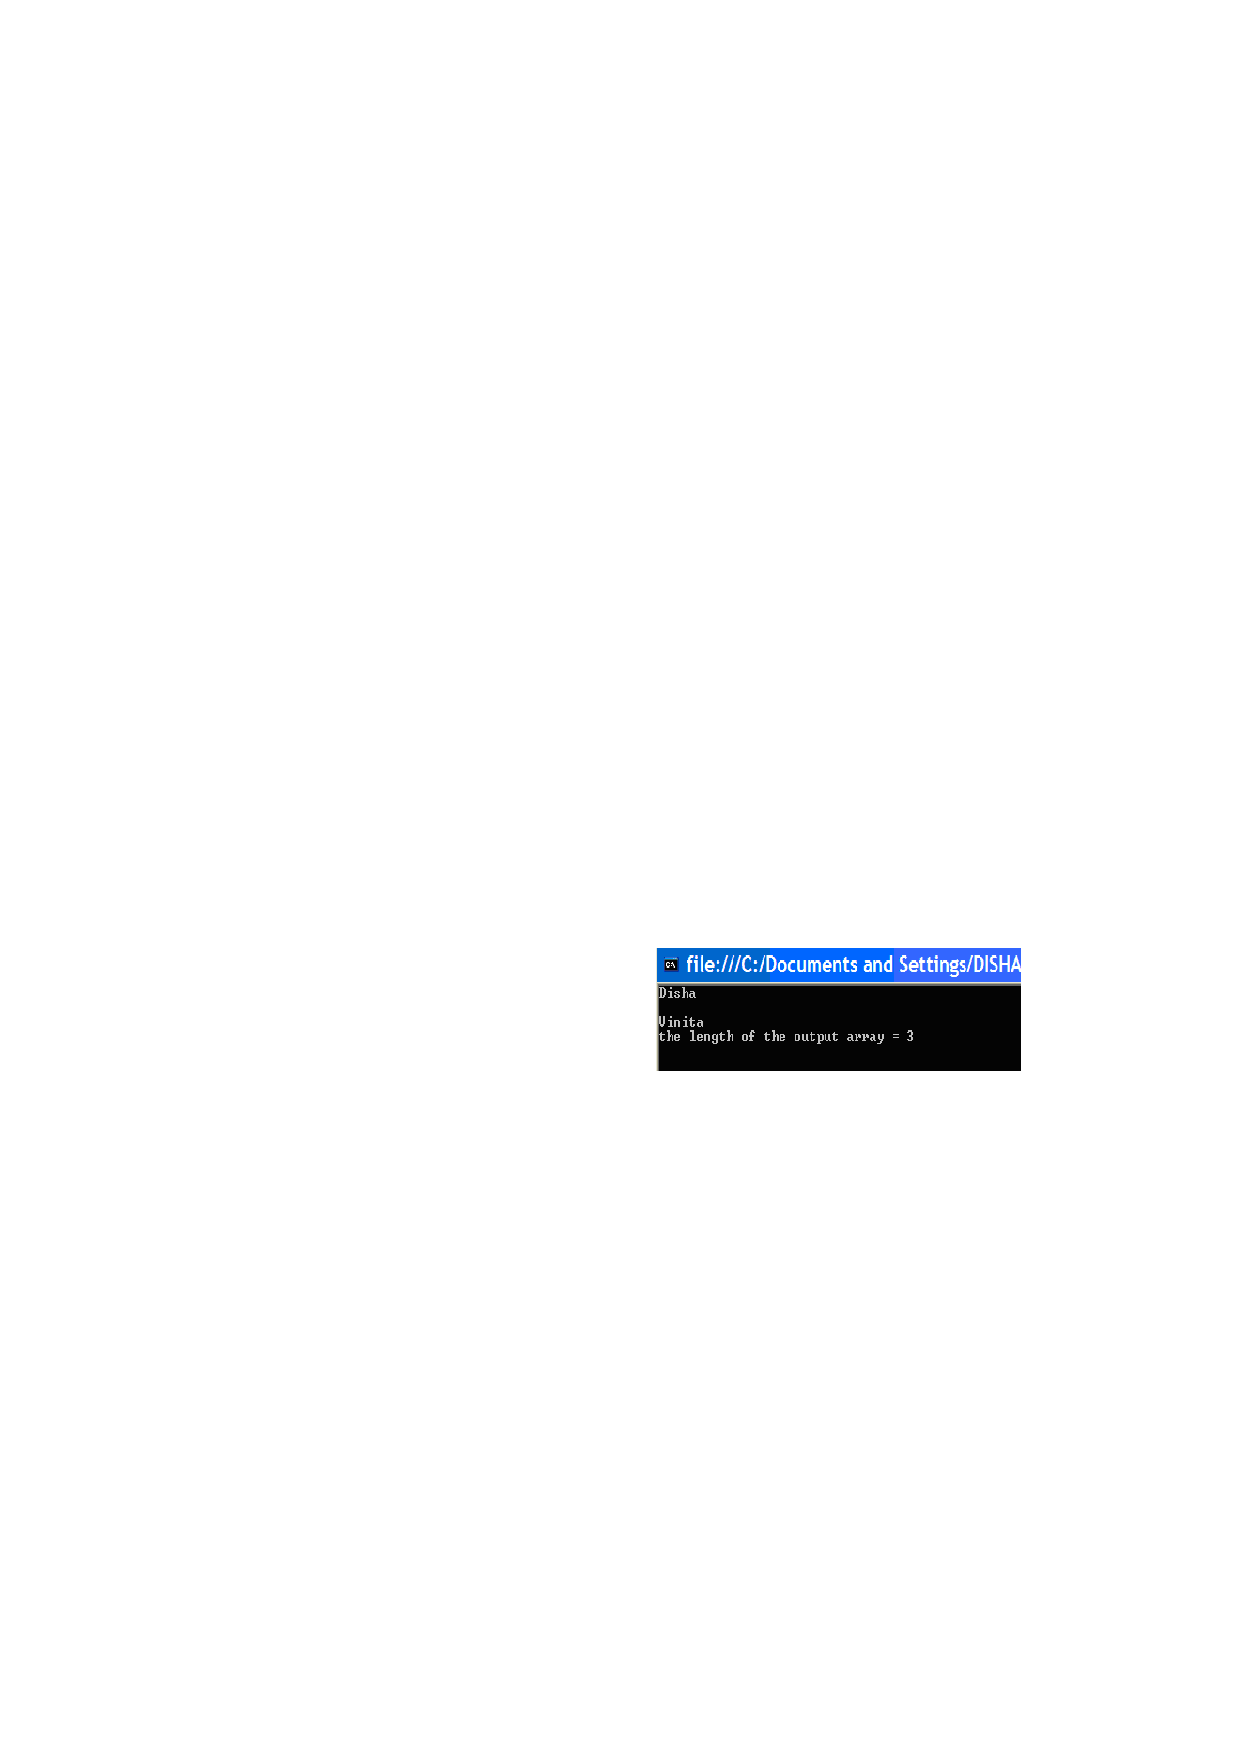
\includegraphics[scale=0.9]{graphics/NETNullSmall.pdf}
  \\ \tiny{images based on Shetty and Vadivel\cite{Shetty:2009}}
  \end{column}
  \end{columns}
\end{frame}
% The different ways languages process data can be a little subtle, and finding differences can require direct testing.
% Shetty and Vadivel looked at Java and .NET web services to find some of these differences


%The difference is most apparent when looking at numbers: Different languages have different default decimal precisions.
%However, this can also show up in other types, such as handling NULL or NIL values

\section[Concepts]{Concepts in interoperability}

\subsection{Metadata}

\begin{frame}
  \frametitle{Metadata and type conversion}

	Metadata: Data about data
	
	or: Information beyond what the data itself can convey
	
	{\tt (def mylist [1, 2, 3, 4])}
	
	{\tt (with-meta mylist \{:length 4, :type Integer\})}
	\linespace
	In Clojure:
	\begin{itemize}
	\item lists are untyped; can contain entries of different types.
	\item metadata use and checking is up to the programmer.
	\end{itemize}
	
	
\end{frame}
%Say we had x = 5. all x knows is that it's a five. "Integer" is a storage mechanism, or representation in the language.
%"Integer" is also context specific. Java knows about x's integer-ness, but JavaScript, or JSON, does not. 

%Metadata can also be used to supply context to data that otherwise would not have it, such as data from a dynamically-typed languge,
%as well as data being sent over a network.

\begin{frame}
\frametitle{Metadata and type conversion}
 \begin{center}
 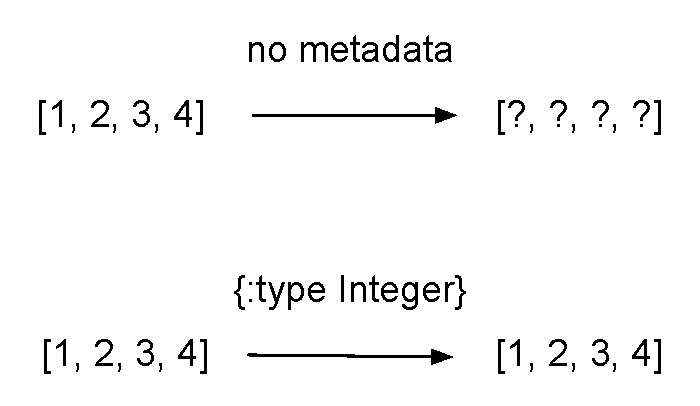
\includegraphics[scale=0.7]{graphics/metadataExample.pdf}
 \end{center}
\end{frame}


\subsection{Standards}

\begin{frame}
  \frametitle{Metadata and standards}
  \begin{center}
  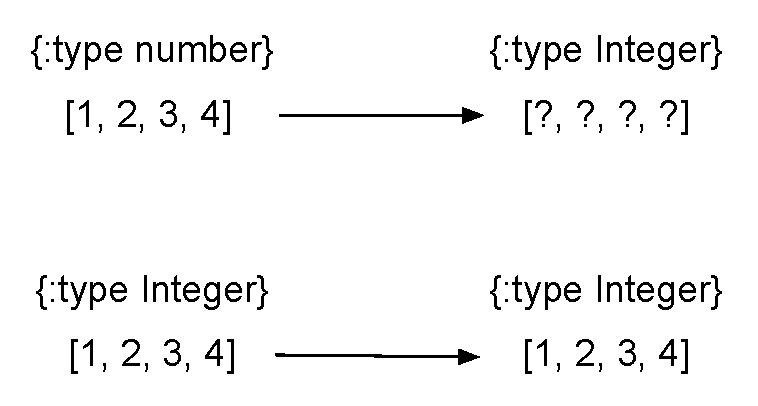
\includegraphics[scale=0.7]{graphics/metadataStandards.pdf}
  \end{center}

  
\end{frame}

\begin{frame}
  \frametitle{The importance of standards}
  \begin{columns}
  \begin{column}{0.6\textwidth}
  Standards are meant to ensure:
  \begin{itemize}
  	\item Agreement on what metadata is being used, and how.
	\item All involved parties know how data will be represented.
	\item Future parties will know how data is represented.
	\item In general, that correct communication happens.
  \end{itemize}
  \end{column}

  \begin{column}{0.5\textwidth}
    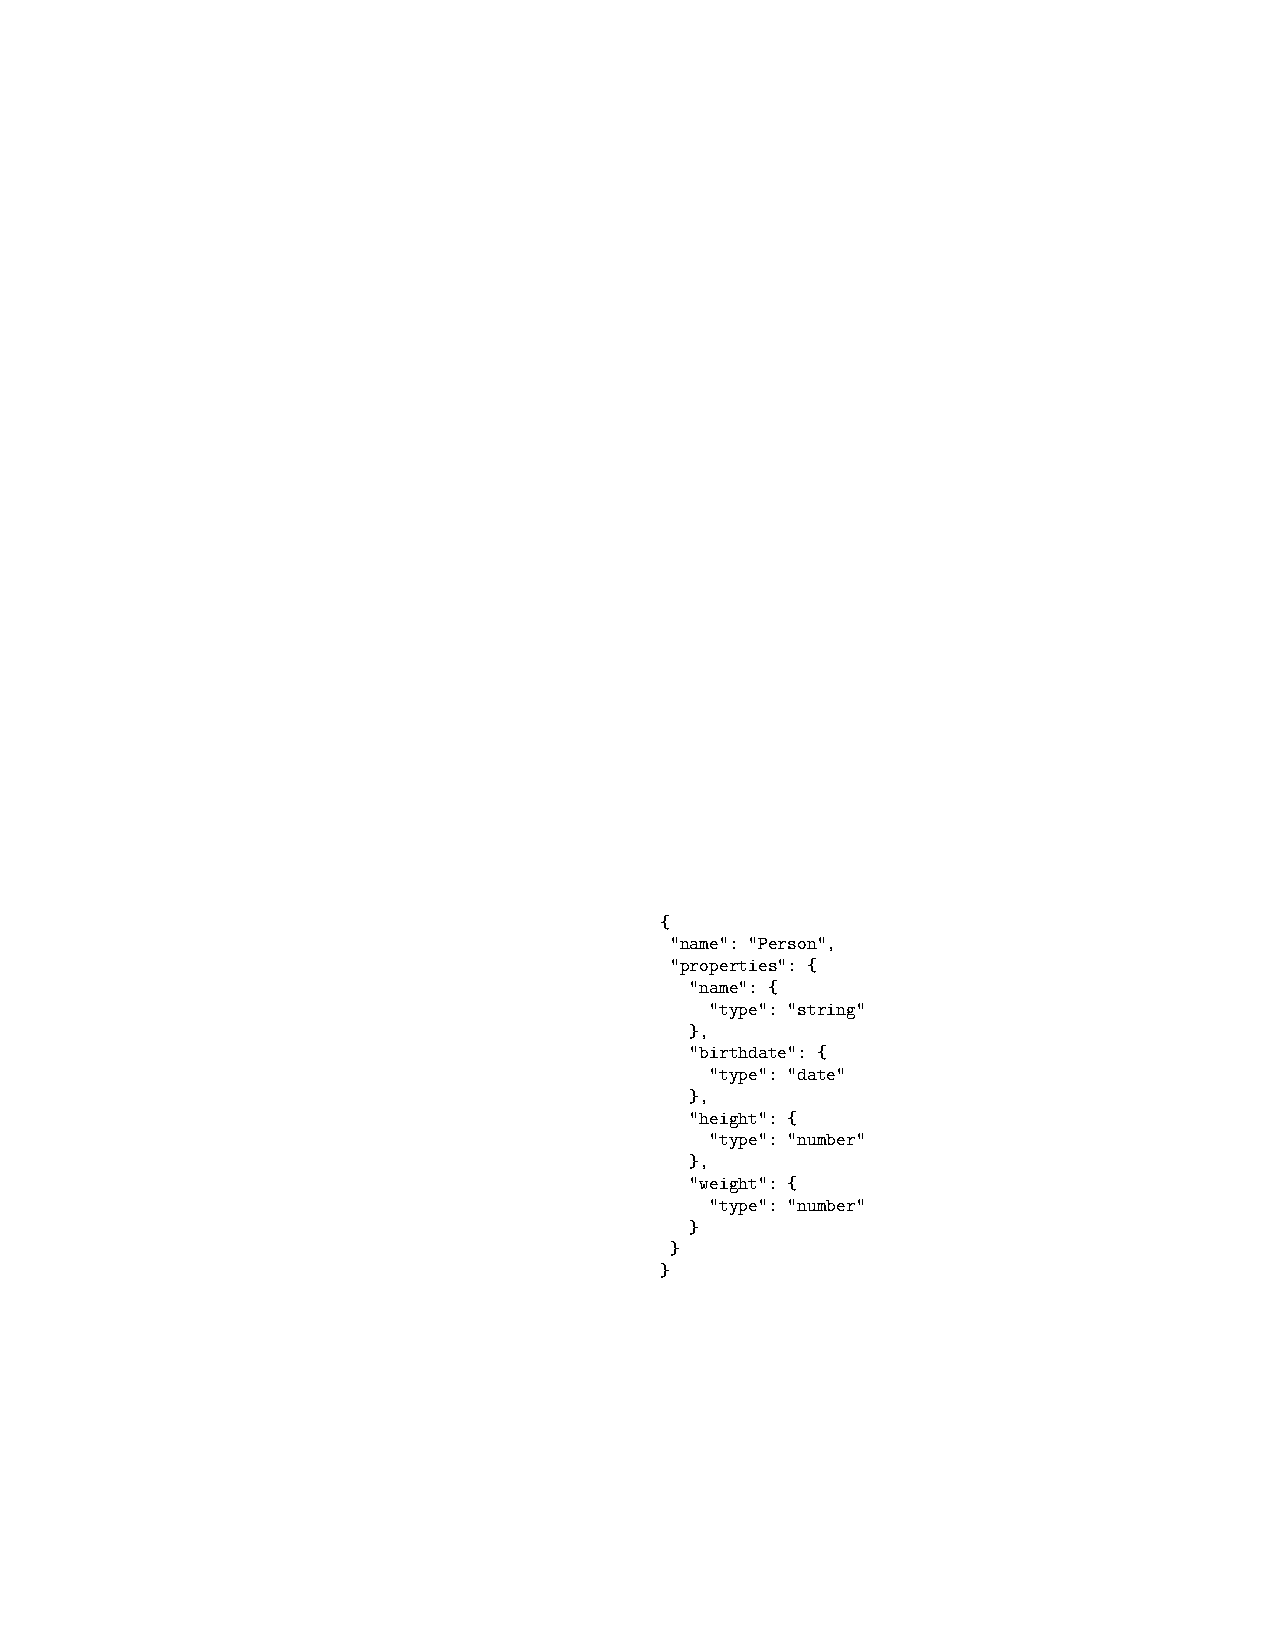
\includegraphics[scale=0.9]{graphics/JSONSchema.pdf}
  \end{column}
  \end{columns}
\end{frame}
%metadata helps us communicate type information; standards help to ensure that all parties are expecting the same expression of type information.
%having a standard also ensures that future parties who want to use the system, or add to the system, will know how to do so gracefully.
%Schema are one way to enforce standards, which we'll discuss later. Schema are tools that can be 

%Metadata ensures that correct communication *can* occur, and standards ensure correct communication *does* occur.


\section[Interop Tools]{Tools used in achieving interoperability}

\subsection{Virtual Machines}

\begin{frame}
  \frametitle{Virtual machines}
  
  %add graphic: CLR VM
  \begin{columns}
  \begin{column}{0.6\textwidth}
  \begin{itemize}
	\item Virtual Machines (VMs) are a runtime environment for a program
	\item High-level languages compile to an intermediate language
	\item Intermediate language: Java bytecode or Common Intermediate Language
  \end{itemize}
  \end{column}
  
  \begin{column}{0.5\textwidth}
  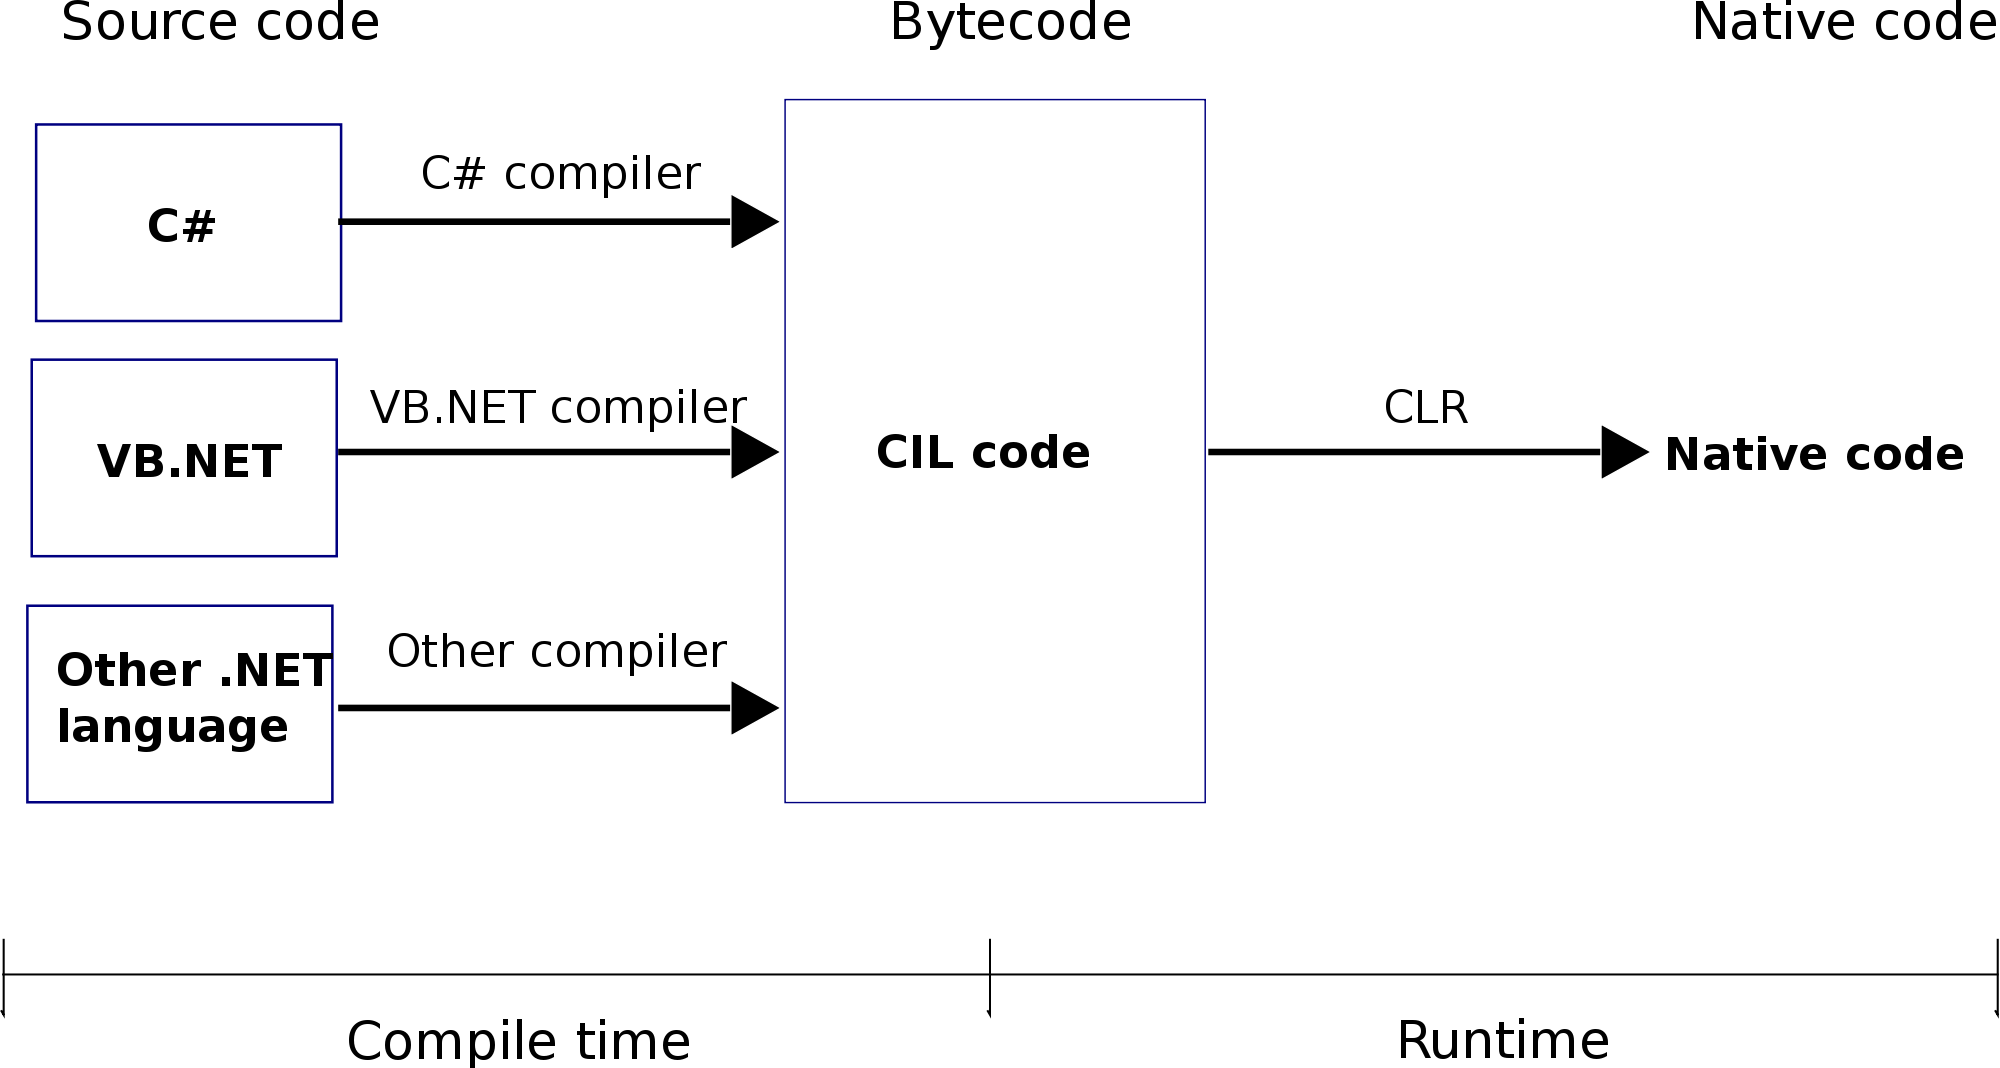
\includegraphics[width=1\textwidth]{graphics/CLR.png}
    \\
    \only{\tiny{Wikipedia \\ \url{https://en.wikipedia.org/wiki/Common_Language_Runtime}}}
  \end{column}
  \end{columns}
\end{frame}
%Briefly, VMs emulate an operating system, or computer hardware. We'll be talking about a specific kind of VM, the process VM, that acts as a runtime environment for a program.
%Once in bytecode, all the parts adhere to the same syntax and language rules, regardless of the high-level language used. They might look different, but...

\begin{frame}[fragile]
  \frametitle{High-level vs Bytecode}
  \begin{columns}
  \begin{column}{0.65\textwidth}
  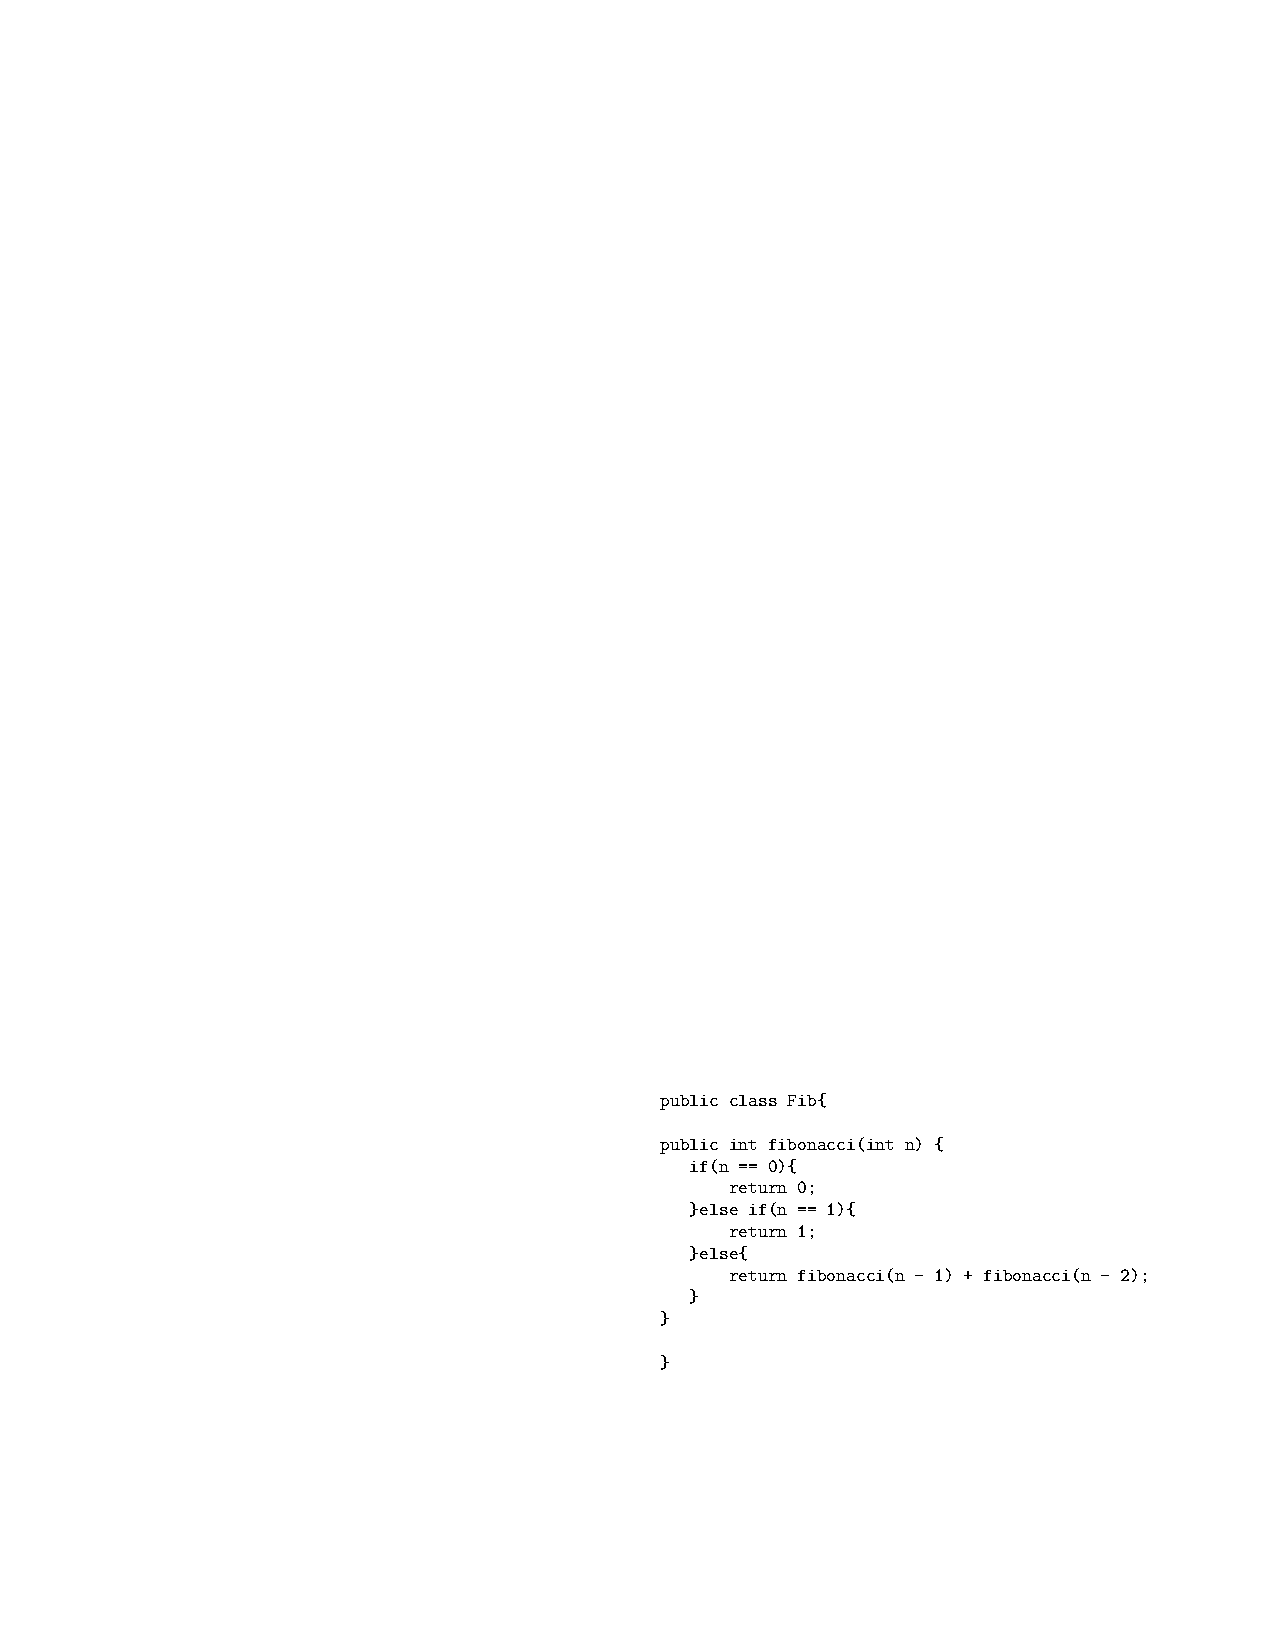
\includegraphics[scale=0.8]{graphics/JavaFib.pdf}
  \end{column}
  
  \begin{column}{0.4\textwidth}
  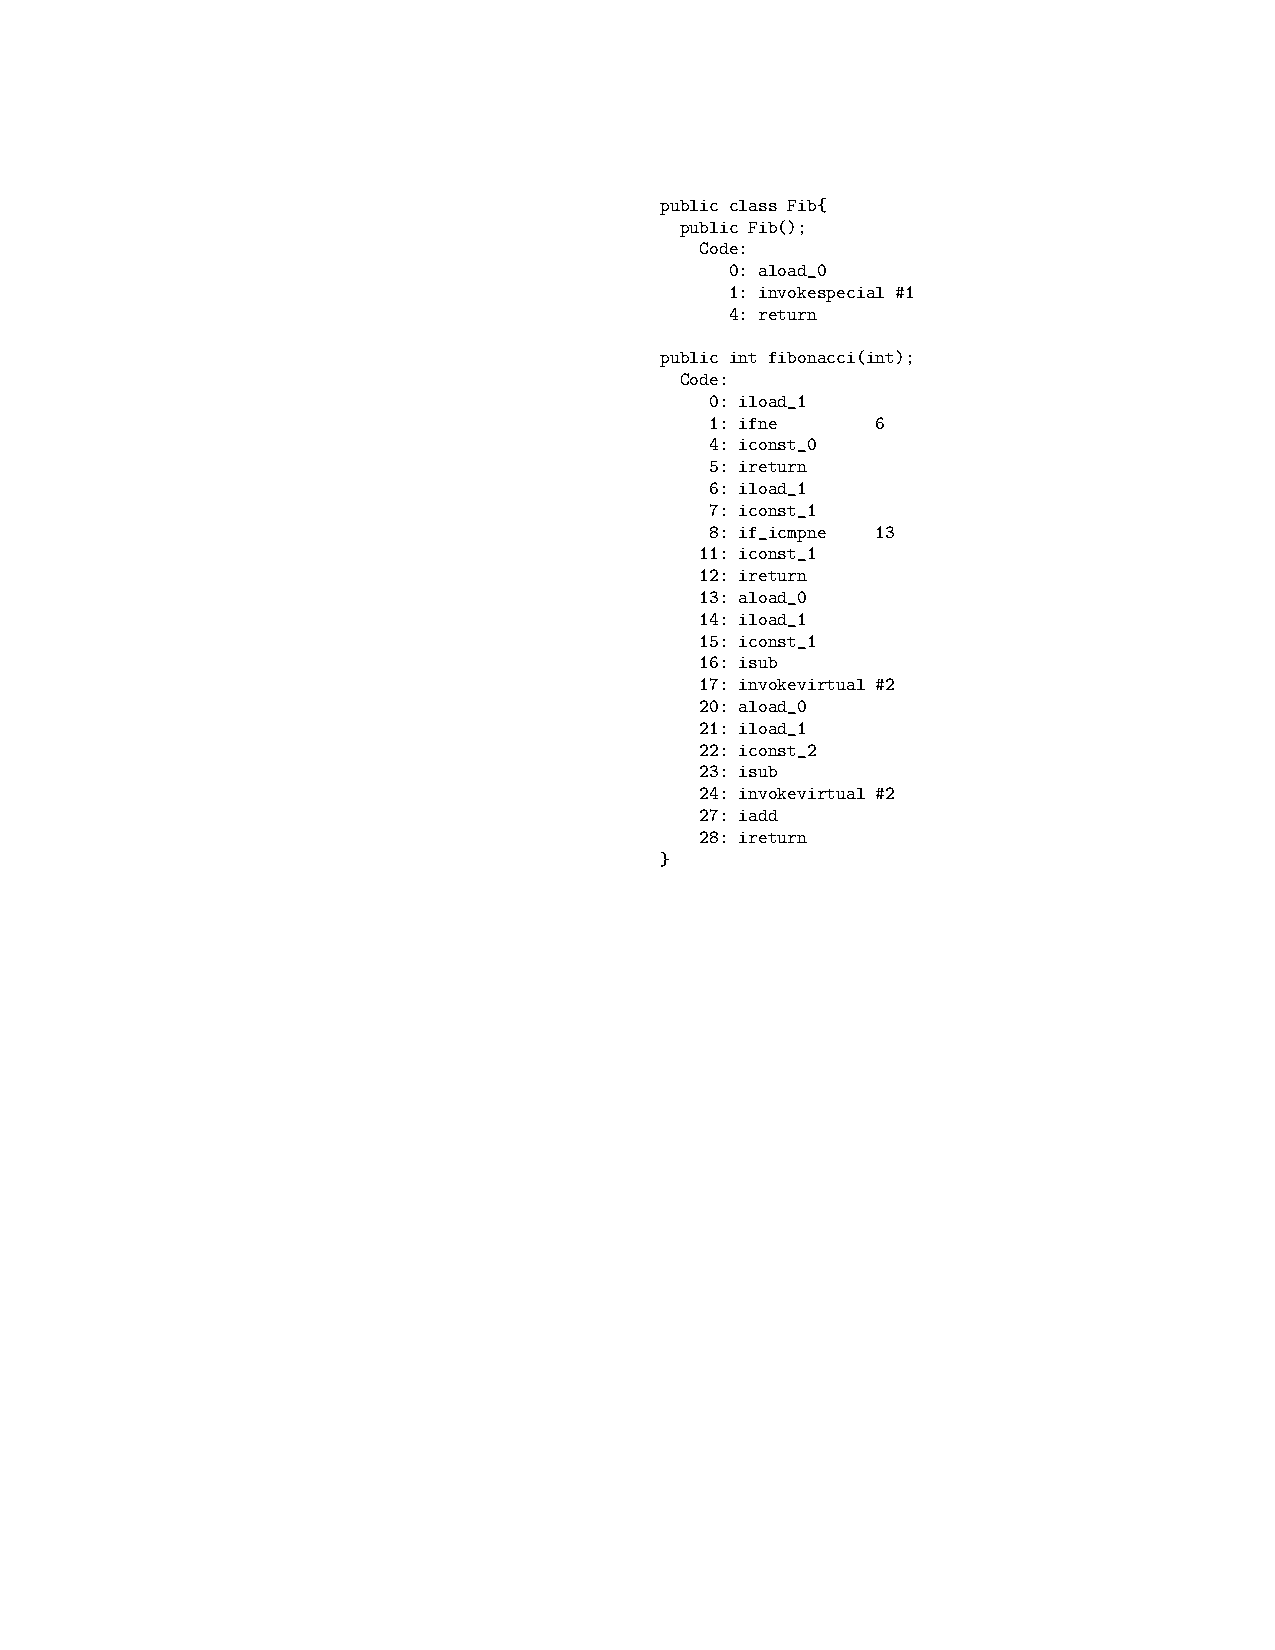
\includegraphics[scale=0.8]{graphics/bytecodeFib.pdf}
  \end{column}
  \end{columns}
\end{frame}

\begin{frame}
 \frametitle{Interoperability with virtual machines}
 \begin{columns}
 \begin{column}{0.5\textwidth}
 \begin{itemize}
 \item Usually some overheard associated with calling other languages.
 \item Overhead can be lessened when all languages are on one VM.
 \item High-level languages can have conventions to call other high-level languages on the same VM.
 \item Common language ensures common syntax and behavior.
 \end{itemize}
 \end{column}
  %Languages on a VM can call one another, as long as they have a calling convention for the other language.
  %This is mainly a syntactic way to access other .class files.
  %There should be no additional overhead, since the actual call will be in the intermediate language
 
 \begin{column}{0.5\textwidth}
 
 A Java method of object cliff:

 {\tt cliff.getAge();}
 \linespace
 \linespace
 \linespace
 Clojure calling Java:
 
 {\tt (. getAge cliff)}
 \linespace
 \linespace
 JRuby calling Java:
 
 {\tt require `java'
 
 cliff.getAge()}
 \end{column}
 \end{columns}
\end{frame}
%Cliff is 36. Both of these would return that
\subsection{Markup Languages}

\begin{frame}
  \frametitle{Markup languages}
  
  \begin{columns}
  \begin{column}{0.5\textwidth}
  \begin{itemize}
	\item Markup languages are a way of modeling data, and act as metadata
	\item XML and JSON can model data like objects.
	\item Markup languages are independent of programming languages.
  \end{itemize}
  \end{column}

  \begin{column}{0.55\textwidth}
   
\includegraphics[scale=1]{graphics/XMLCliff.pdf}
   
   \tiny{XML model of a person}
   \linespace
   \linespace
   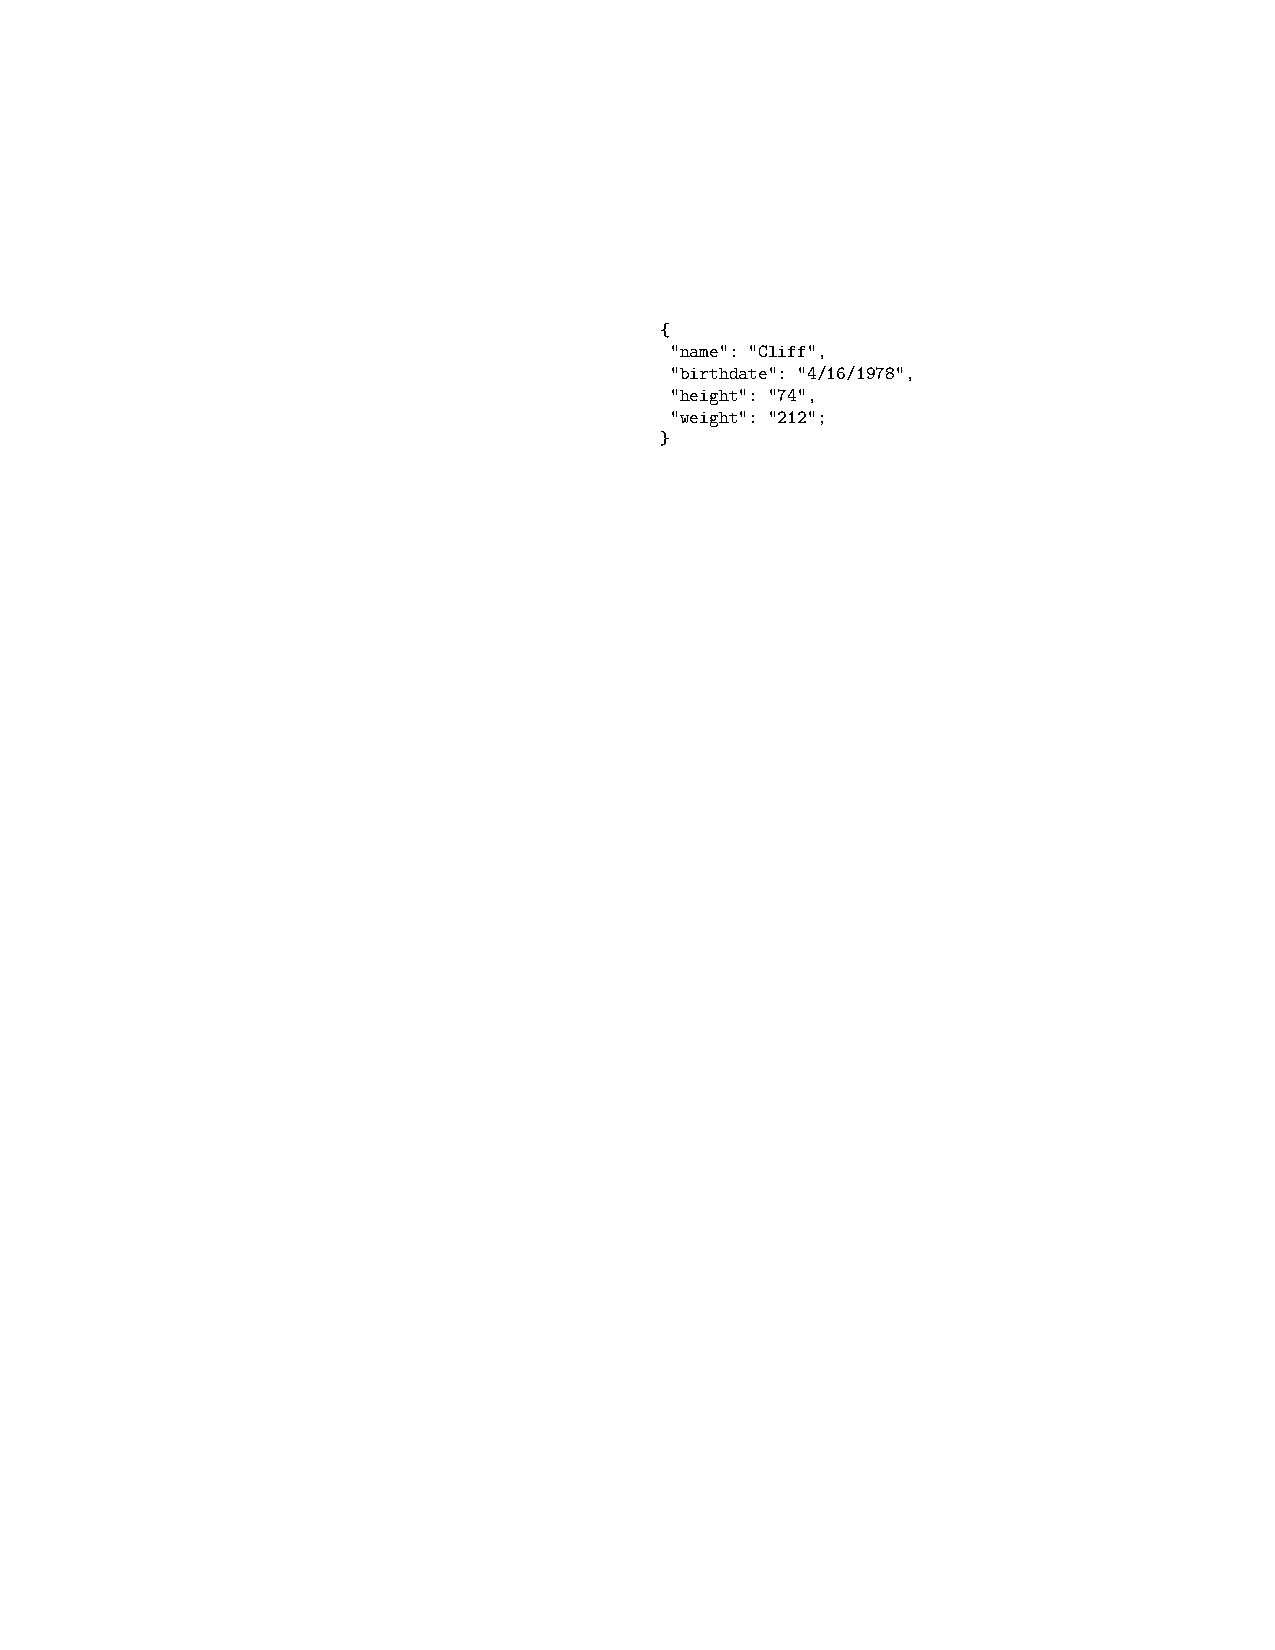
\includegraphics[scale=1]{graphics/JSONCliff.pdf}
   
   \tiny{JSON model of a person}
  \end{column}
  \end{columns}
  
\end{frame}
%MLs are mostly a way of annotating data in a way that another program can interpret that meaningfully, handle it accordingly.
%one of the emergent properties of this, in the form of XML, is the ability to model data in a way that it can be converted to a data structure in the reciving program.
%Several other languages have emerged to model data specifically in this way, like JSON. JSON is JavaScript's Object Notation, implying correctly that it models data like an object.

 \begin{frame}
  \frametitle{Schema and standardization}
  \begin{columns}
  \begin{column}{0.5\textwidth}
  \begin{itemize}
  \item Schema provide both standardization and additional metadata.
  \item Libraries exist to check incoming data against a schema.
  \end{itemize}
  \end{column}
  
  \begin{column}{0.66\textwidth}  
  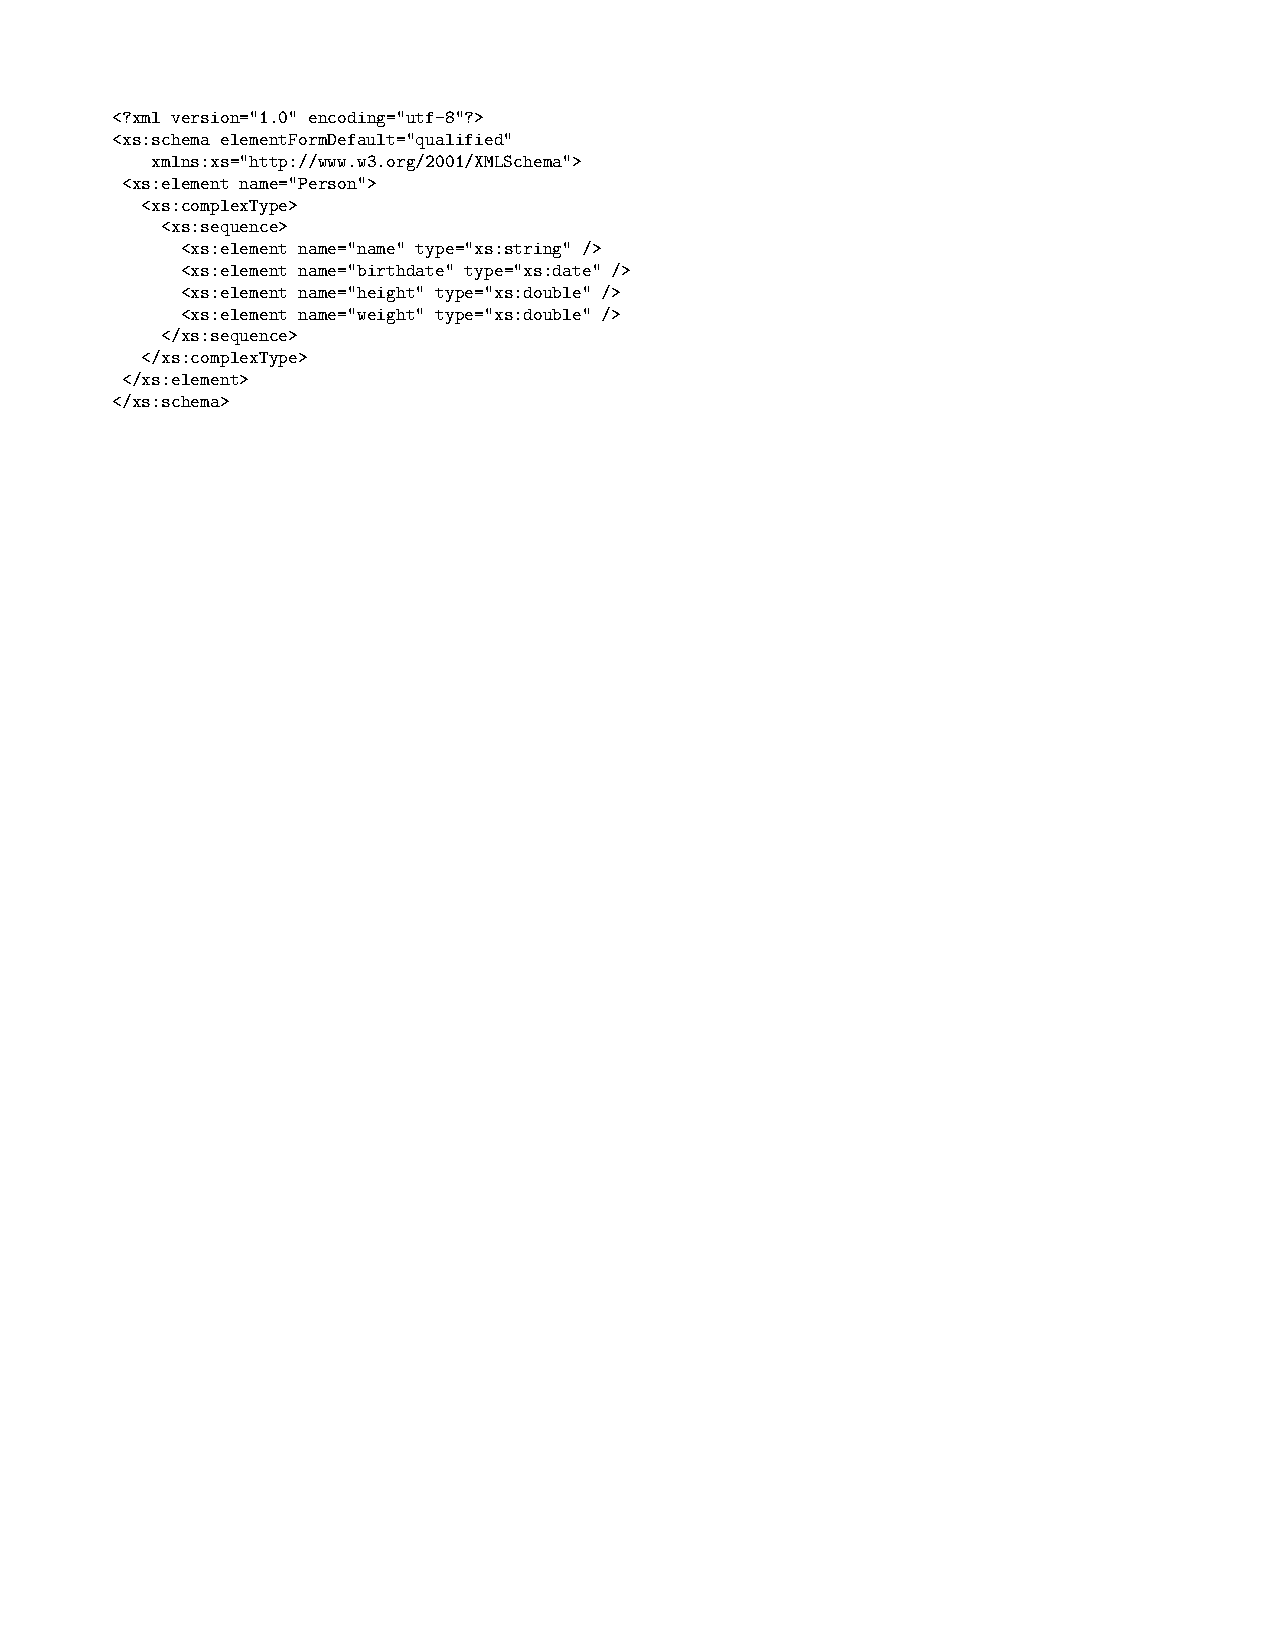
\includegraphics[scale=0.8]{graphics/XMLSchemaW3C.pdf}
  \end{column}
  \end{columns}
 \end{frame}
%MLs are most useful when data will be decontextualized for whatever reason
%Since MLs can act as metadata

 \begin{frame}
 \frametitle{Client/server interop with markup languages}
 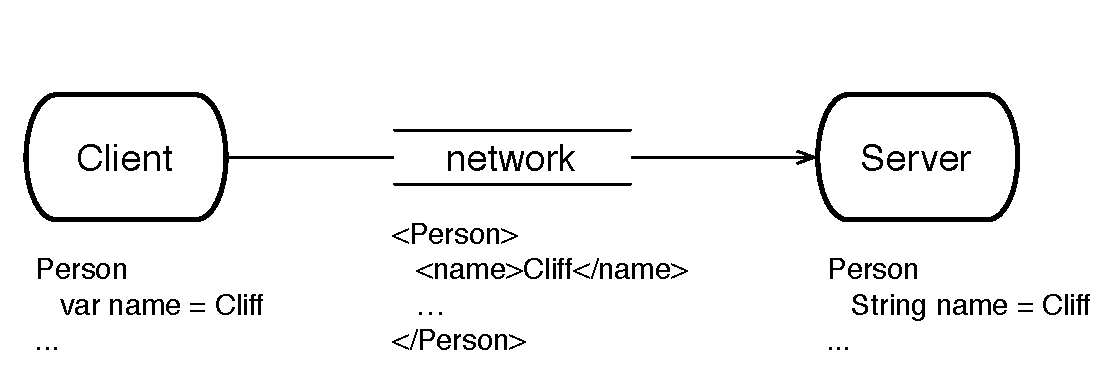
\includegraphics[scale=0.6]{graphics/ClientServer.pdf}
 
 Communication across a network using XML
 
 \end{frame}

\section[Conclusions]{Conclusions}

\begin{frame}
  \frametitle{Conclusions}
  \begin{itemize}
  	\item Interop allows programmers to extend existing systems without requiring them to know the original language.
  	\item Also allows programmers access to the strengths of languages other than the main system language.
	\item Metadata and standards allow programmers to reason about interoperability, and to communicate how their system handles interop.
	\item Virtual machines and markup languages make use of these concepts to enable interop.
  \end{itemize}
\end{frame}




\begin{frame}
	\frametitle{Thank you for listening!}
		

	\linespace
	\linespace
	\linespace
	
	\begin{center}
	{\huge Questions?}
	\end{center}
	
    \linespace
	\linespace
	\linespace
	
	Contact:  
		\texttt{malone153@morris.umn.edu}
\end{frame}

\section*{References}

\begin{frame} 
	\frametitle{References} 
	
	\bibliographystyle{abbrv}
	\bibliography{bibliography}
	
\end{frame} 

\end{document}


